\documentclass[a4paper, 12pt]{memoir}
\usepackage{a4wide}
\usepackage{fontspec}
\usepackage[french]{babel}
\usepackage{graphicx}
\usepackage{amsfonts}
\usepackage{amsmath}
\usepackage{xcolor}
\usepackage{pdfpages}  % pour la page de garde

\usepackage{mathtools}
%\usepackage{varioref}

% lien hypertextes:
\usepackage[colorlinks=true,citecolor=blue]{hyperref}

% Le plan va jusqu'à la subsection
\setsecnumdepth{subsection}

% ------------- apparences (pfff, ce que c'est futile tout ça)
% font
\defaultfontfeatures{Mapping=tex-text}
\setmainfont{Linux Libertine O}
% style de chapitre
\chapterstyle{bianchi}
% style des headers
\setsecheadstyle{\sffamily\Large\bfseries}
\setsubsecheadstyle{\sffamily\large\bfseries}
% style des captions
\captionnamefont{\sffamily\bfseries\tiny}




% ------------- ma pwn macroz
\newcommand\introduceterm[1]{\textcolor{purple}{#1}{}}

 
%\title{Mathonomicon, vol. 1: 101}
%\author{Le Muchacho Masqué}

\begin{document}
\thispagestyle{plain}
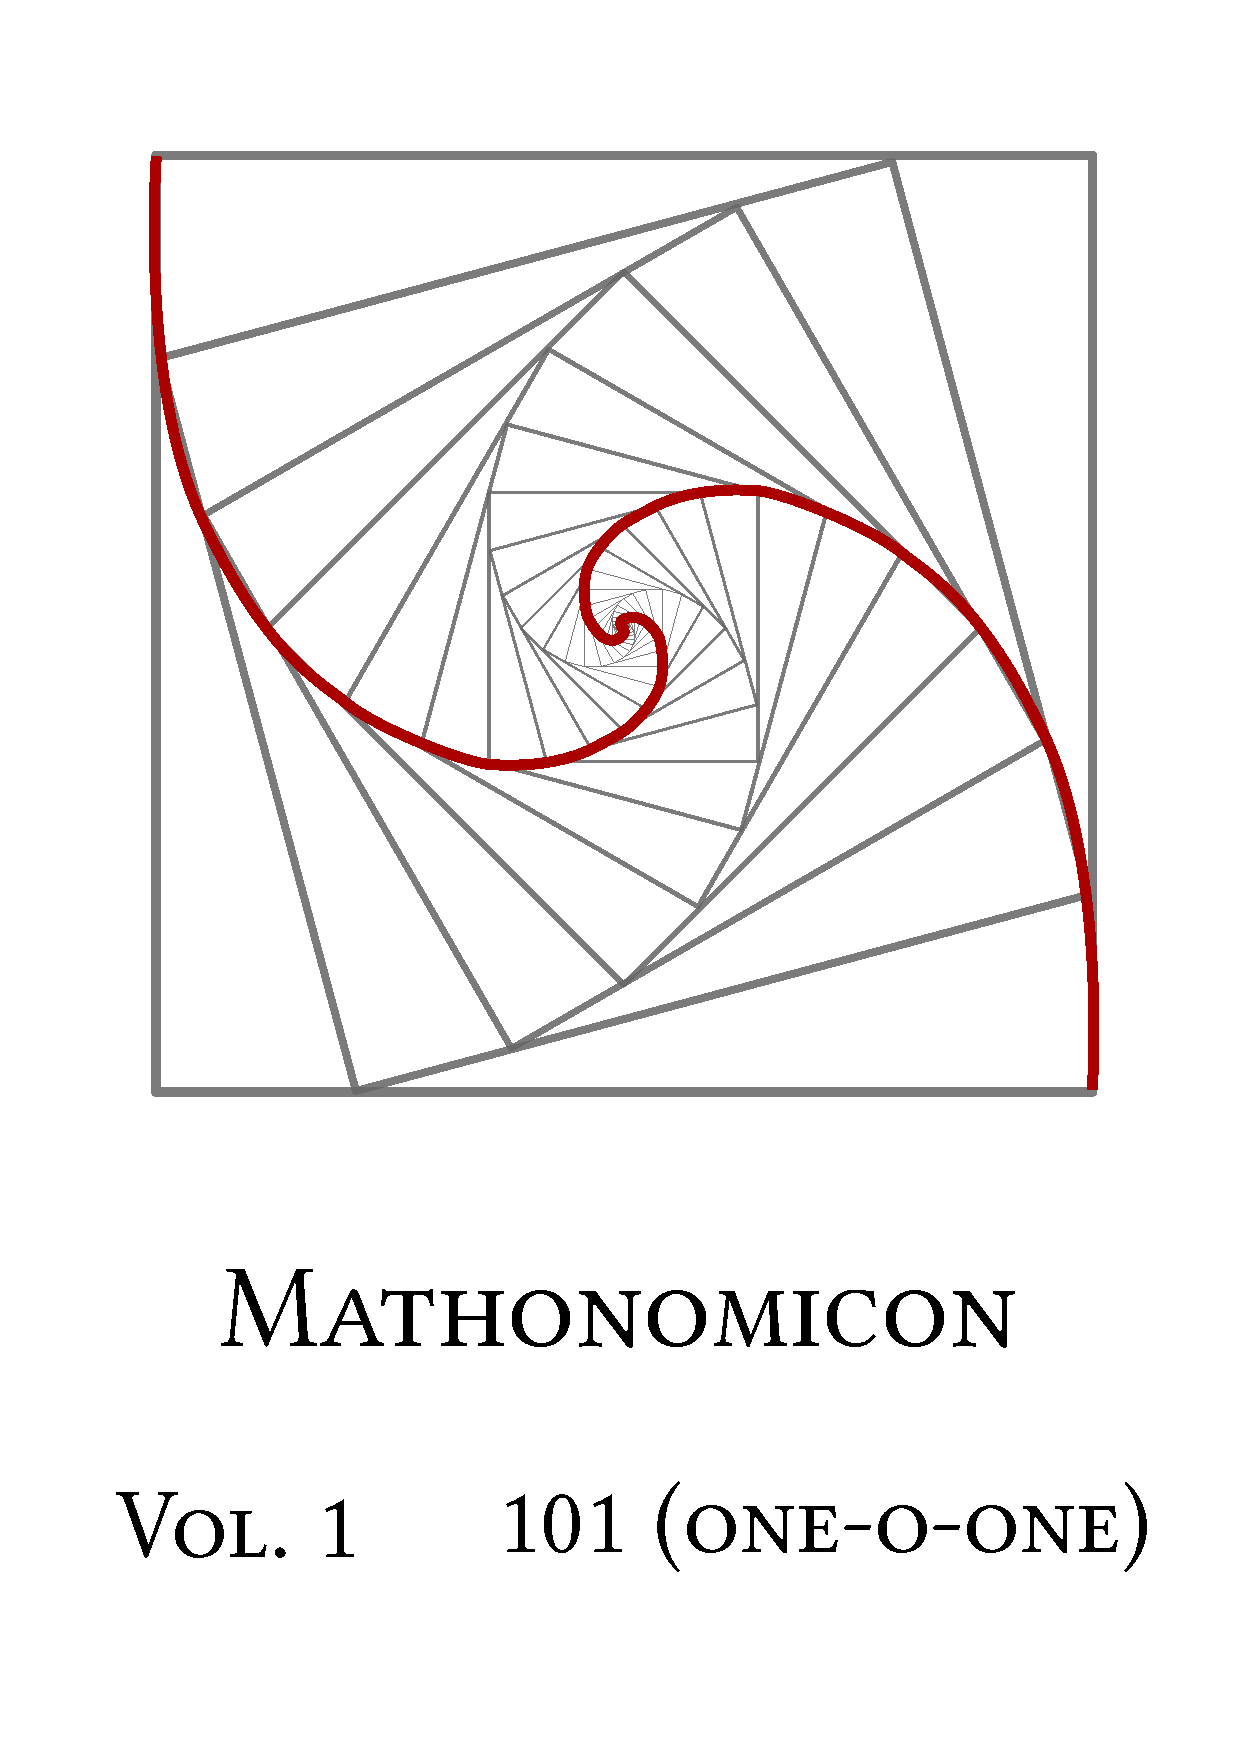
\includepdf[pages=1]{page-de-garde.pdf}

\newpage

\tableofcontents

\chapter*{Introduction}
\addcontentsline{toc}{chapter}{Introduction} 

Comme les plus perspicaces d'entre vous l'auront compris en lisant le
titre du présent document, il s'agit ici de parler de maths. Pourquoi
donc ? Les mathématiques sont je pense laissées de côté de nos
jours. Non pas dans le sens où peu de gens les étudient: rien ne
serait plus faux. Je parle de la quasi-absence de vulgarisation en la
matière. Alors qu'il ne pas difficile de trouver des ouvrages de
vulgarisation de physique rendant accessibles des concepts aussi
alambiqués que la relativité générale à tout être de bonne volonté, on
ne peut que déplorer l'absence de médias équivalents pour les
mathématiques. Par ailleurs, la façon dont elles sont présentées dans
le système français,\footnote{D'un autre côté, ce n'est pas forcément
  beaucoup mieux ailleurs d'après ce que j'ai vu.} bien qu'ayant des
vertues pédagogiques indéniables et permettant de donner rapidement
les outils de base pour les calculs de la vie courante, ne donne pas,
à mon sens, une vision de ce que sont vraiment les mathématiques. Tout
au plus apprend-on une série de recettes de cuisine nous permettant de
résoudre des problèmes bien précis. Certes cela peut d'avérer
utile. Certes encore il se trouve des gens pour considérer que c'est
faire des maths que de faire cela. Il n'en reste pas moins que réduire
ce domaine des sciences à cela est \emph{un poil} réducteur. D'autant
plus que cette partie est loin d'être la plus intéressante.

Avant de terminer mes élucubrations d'une légitimité douteuse sur la
qualité de l'enseignement des maths, sachez qu'il n'est absolument pas
nécessaire d'avoir des connaissances de bases pour lire ce
livre. Gardez également à l'esprit que, quand bien même vous auriez eu
du mal à suivre les cours que vous aviez à l'école, le contenu ici est
différent. Du coup, même si vous aviez du mal, j'ai bon espoir que
vous me compreniez. À la condition bien évidemment que vous y mettiez
du vôtre.\footnote{Non parce que sinon vous pouvez toujours courir: la
  connaissance ne va vous tomber toute seule dans le bec! Ah, mais!}


Une autre des motivations qui m'ont poussé à écrire ce
\emph{mathonomicon} vient du constat que la connaissance donne le
pouvoir. La contraposée est tout particulièrement vraie : l'absence de
connaissance entraîne l'absence de pouvoir. Il est infiniment plus
facile de manipuler une personne en l'entraînant sur un terrain
qu'elle ne connaît qu'en la laissant parmi les éléments qu'elle
maîtrise. Par exemple, l'utilisation politique actuelle des
statistiques\footnote{En dépit du fait qu'il ne s'agisse pas vraiment
  de mathématiques, j'ai décidé de traiter (fort superficiellement, je
  suis tout sauf un spécialiste en la matière) le sujet ici au motif
  que quand même, ça sert pas mal ces trucs.} fait bondir n'importe
quelle personne ayant un tant soit peu de connaissances sur le
sujet. Par exemple, corrélation n'est pas causalité; mais j'y
reviendrai en temps utile.


Plus généralement, la pensée mathématique est à la base de la pensée
scientifique. Par conséquent, une fois que vous aurez pris le ``coup
d'esprit'' (on ne peut pas vraiment parler de coup de main), vous
serez à même de porter un regard critique sur les discours
``scientifiques'' des différents illuminés capables d'affirmer, par
exemple, que la fin du monde est pour 2012, ``preuve à
l'appui''. Affirmer qu'une chose est vraie sans pouvoir le démontrer,
c'est en réalité ne rien dire. Les matheux le savent mieux que
quiconque, eux dont le cœur de métier est de précisément de démontrer
de nouveaux théorèmes. J'espère sincèrement que vous serez convaincus
de cela après avoir lu le mathonomicon et, surtout, j'espère que vous
saurez juger efficacement de la qualité d'une argumentation au sens
strictement logique, sans tenir compte des artifices réthoriques.


Un autre intérêt bassement pragmatique de la connaissance des
mathématiques provient d'un constat très simple: un autre ordinateur
n'est rien de plus qu'une machine à calculer. Il n'est rien de moins
non plus. Par conséquent, pour espérer comprendre comment fonctionne
ces bestioles à un niveau plus avancé que ``lolilol facebook et msn
c'est trop bien'',\footnote{Allons, on en connaît tous des comme
  ça. C'est pas grave hein, on les aime quand même. Même s'ils sont
  très vilains. Parce qu'ils sont très très vilains, hein!} il
est extrêmement utile d'avoir de bonnes bases en maths. En fait, si
vous voulez vous mettre sérieusement à l'administration de systèmes
ou, pire, à la programmation, il est impensable de ne pas avoir un
bagage suffisant en maths

Pour toutes ces raisons, je me suis lancé dans la folle entreprise de
rédiger un document se voulant une bible des matheux. Non pas dans le
sens où il contiendra toutes les connaissances actuelles car une vie,
la mienne en l'occurrence, n'y suffirait. En fait, je l'envisage comme
un moyen de fournir à tout un chacun un aperçu de l'étendue réelle des
mathématiques. Plus même qu'un aperçu, j'ose croire fournir également
les bases théoriques qui permettent une compréhension réelles des
résultats évoqués: il ne s'agit pas de savoir réciter les théorèmes
que je mentionne tout au long du mathonomicon mais bien de les
intégrer, des les intérioriser presque à tel point que vous ne
réfléchirez même plus avant des les utiliser. Vous remarquerez
immédiatement les confusions entre contraposées et réciproques et vous
penserez à des structures algébraïque quand on vous parlera
d'anneaux. Un autre avantage, c'est que vous pourrez vous extasier sur
la complexité de ce qui vous entoure. Vous ne pourrez plus manquer la
dimension fractale des côtes de Bretagne et vous apprécierez à leur
juste valeur les algorithmes qui vous ont permis de télécharger ce
document. Cette capacité à remarquer une beauté que tant ignore est je
trouve infiniment précieuse.


Qui suis-je donc pour parler de la sorte ? Laissez-moi moi contourner
habilement cette question on vous contant une histoire. Une histoire
on ne peut plus vraie car facilement vérifiable (les moteurs de
recherche sont vos amis). Vous n'êtes probablement pas sans avoir
qu'il y a de cela plusieurs dizaines d'années nous nous somme
joyeusement entre-tués à l'échelle mondiale, qui coulant des bateaux
dans l'Atlantique depuis son sous-marin, qui massacrant avec force
enthousiasme des centaines de civils à Beijing, qui enfin recouvrant
une ville de dispositifs explosifs déclenchés par simple
contact.\footnote{U-boat pendant la bataille de l'Atlantique, sac de
  Pékin et n'importe quel bombardement de n'importe quel ville par
  n'importe quelle alliance pour ceux qui auraient du mal à suivre mes
  allusions.} Avant même que l'on en arrive là, les Polonais avaient
un mauvais pressentiment vis-à-vis de leur voisin Germain. De plus,
celui-ci avait pris durant les années 20-30 l'habitude de chiffrer ses
communications, c'est à dire d'appliquer une transformation
mathématique à ses messages de façon à les rendre inintelligibles pour
quiconque les intercepterait. Le processus était bien évidemment
réversible pour peu que l'on connaisse une certaine clé, c'est à dire
\emph{grosso modo} un mot de passe. Les Polonais, et l'avenir prouvera
qu'ils ont bien fait, ce sont donc attelés à la tâche de décoder ces
messages sans connaître ne serait-ce que le fonctionnement exact de la
machine utilisée par les Allemands. Et bien évidemment, sans avoir
\emph{a priori} aucune information sur les clefs utilisées. Cela peut
sembler difficile mais ce serait en réalité un doux euphémisme que de
dire cela: les mathématiques impliquées (études des permutations) ne
sont pas franchement triviales et, même en ayant les connaissances
adéquates, il faut encore avoir les idées et la créativité nécessaires
à la découverte d'une solution. Lors donc, un mathématicien polonais,
Marian Rejewski, à force d'astuces, de perséverance\footnote{Et aussi
  en corrompant un officer allemand. Parce que oui, des fois on peut
  tricher.} et d'innovation est parvenu à percer cette protection des
messages. Non seulement il a compris le fonctionnement de la machine
utilisée par les Allemands, ENIGMA mais il a également conçu et
construit des machines en automatisant le décryptage: les premières
bombes cryptographiques. Ces machines sont les ancêtres des
ordinateurs tels que celui que vous utilisez pour lire ce tome du
Mathonomicon. Néanmoins, le passage d'une machine spécialisée à une
machine programmable pouvant accomplir est le fait d'un autre génie,
plus connu, Alan Turing. Mais revenons à notre ami Marian. Juste avant
que les nazis envahissent la Pologne, il fuit en direction de la
France (alors encore libre) et y rencontra justement M. Turing à qui
il présenta ces travaux et le fonctionnement de ses bombes
cryptographiques. Turing compris la leçon et retourna en Angleterre, à
Bletchey Park où il industrialisa la cryptanalyse d'ENIGMA: les alliés
connaissaient ainsi en temps quasi-réel des messages que les Allemands
croyaient naïvement sécurisés. D'où victoire dans la bataille de
l'Atlantique (c'est facile de couler des U-boats quand on sait où ils
sont) puis, moins directement certes, victoire des alliés. Tout cela
grâce à une bande de mathématiciens parmi lesquels seul Turing, père
de l'informatique, deviendra (un peu) célèbre. Marian retournera en
Pologne et vivra dans le plus complet anonymat pendant des
années. Tout au plus y'a-t-il \emph{une} statue à sa gloire, quelque
part en Pologne. Pourtant, qui sait ce que nous serions s'il n'avait
pas été là?

Je ne prétends pas combattre le nazisme en écrivant et en diffusant
librement le Mathonomicon. Mais j'ose croire que j'accomplis une bonne
action. Qui sait, peut-être aidera-t-il un jour à un jeune
cryptanalyste à déchiffrer les communications d'une dictature? Je
pense que je ne pourrais pas rêver plus belle récompense pour le
travail que j'ai fourni ici.  Néanmoins, comme l'histoire de Marian
Rejewski le montre,\footnote{Parce que vous croyiez que je vous avait
  raconté tout ça pour la déconne ?} il n'est pas besoin d'être
reconnu pour ses bonnes actions pour que celles-ci aient de la
portée. Par conséquent, estimant mon identité de peu d'intérêt quant à
la pertinence de ce document, je ne vous la donnerai
pas. Nananère-euh. Tout au plus saurez-vous que je suis un matheux
versé dans une moindre mesure dans d'autre sciences, d'où des exemples
que j'espère variés pour illustrer les différents concepts que je
présente ici. Un lecteur patient et motivé pourrait cependant
probablement me retrouver sans trop de difficultés en recoupant les
informations que je laisse immanquablement transparaître ici. Si ça
l'amuse, je n'y voit pas d'inconvénients.


Le Mathonomicon se découpe en deux tomes. Le premier, ``101''
\footnote{Prononcez ``ouane-o-ouane'', à l'anglaise. Il est de coutume
  de donner le numéro 101 au cours d'introduction dans les universités
  américaines.} présente les concepts que j'estime basiques non pas
dans le sens où ils sont faciles d'accès, même si cela s'avère être le
cas, mais dans le sens où ils sont aux fondations de la construction
des mathématiques. Le second, ``Serious Business'' passe au niveau
supérieur et aborde des thèmes plus complexes tout en approfondissant
ceux déjà traités. Toutefois, si vous lisez le second après le
premier, tout se passera bien.

Vous pouvez lire ce document dans l'ordre, auquel cas vous profiterez
de la progression logique et de la difficulté progressive des thèmes
abordés que je me suis évertué à mettre en place. Si vous vous
intéressez à un sujet plus spécifique, vous trouverez en figure
%\ref{fig:dag-dependances}
un ``GOA\footnote{Graphe Orienté
  Acyclique. Vous verez cela bientôt!} de dépendances'', c'est à dire
une représentation schématique des chapitres pré-requis pour un
chapitre donné. 


La progression logique évoquée précédemment est très proche de celle
de mon cours de maths de première année de prépa, que mon professeur
de l'époque soit remercié ici. Certes, un remerciement anonyme n'est
pas follement impressionant mais on ne me taxera pas d'ingratitude. Le
nom même de cet ouvrage est une référence direct au Cryptonomicon,
livre fictif mentionné dans le roman Cryptonomicon de Neal
Stephenson. Le Cryptonomicon, tel que décrit dans ce roman (à qui il a
donné son nom, vous suivez?\footnote{Yo dawg! I heard you like books
  so I put a Cryptonomicon in your Cryptonomicon so you could read
  while you read!}) est un livre écrit à plusieurs mains décrivant
l'état de l'art de la cryptographie. Je ne prétends cependant pas
décrire l'état de l'art des mathématiques ici, encore une fois ma vie
n'y suffirait pas. Ce nom est lui-même une référence au Necromicon
évoqué par Lovecraft. Je serais extrêmement flatté si ce livre servait
à invoquer Cthulhu mais je n'y crois pas trop.

Enfin, au niveau de la forme, sachez que j'ai fait de mon mieux pour
maintenir un certain humour. Ne soyez donc pas surpris si certains
exemples sont bizarres, cocasses, voire franchement débiles. Ils n'en
sont pas moins pertinents. En théorie. Le \emph{Poignant's guide to
Ruby}, pour ceux qui connaissent, m'a donné l'idée de traiter le sujet
sans me prendre au sérieux voire même en pétant volontier un câble
de-ci de-là. Puisse son auteur en être remercié. J'ai gardé les vrais
noms des concepts que je décris et ceux-ci peuvent être intimidant. Ne
vous laissez pas faire et lisez tout de même: vous leur montrerez
bientôt qui est le patron. Enfin, de bonnes âmes n'ont pas manqué de
me relire; qu'il s'agisse de corriger mon orthographe périclitante ou
de ``tester'' une analogie explicative. Qu'elles trouvent ici toute ma
gratitude et toutes mes excuses pour la petite part de santé de
mentale qu'elles n'auront pas manqué de perdre dans le procédé. J'ai
tâché de citer mes sources lorque je me souvenais d'où j'avais pris
telle ou telle notion. Néanmoins, il est fort probable que les-dites
sources soient en anglais: mes plus plates excuses aux lecteurs
exclusivement francophones.

Je pense avoir suffisamment blablatté et je tiens à assurer les
lecteurs parvenus jusqu'ici de mon plus profond respect. Néanmoins,
passons sans plus attendre aux choses sérieuses.


\chapter{Briques de base}
Le présent chapitre étant le premier, je m'en vais commencer par le
commencement. En l'occurrence, l'algèbre Booléenne est au cœur de la
pensée mathématique. Les notions d'équivalence, d'implications, de
conjonction, etc. sont tous simplement incontournables aussi nous
n'allons pas essayer de les contourner. Une fois la logique booléenne
aquise, on corsera le tout en raisonnant sur des ensembles d'abord de
façon intuitive puis plus rigoureusement en utilisant des
quantificateurs. Ensuite, on utilisera ces magnifiques outils
conceptuels pour construire les entiers (le genre de truc qui est
vaguement utile puisqu'il se trouve absolument au \emph{centre} des
maths) et pour voir la notion de fonction (qui est à ranger juste à
côté des entiers).

\section{Algèbre Booléenne}


Nommée ainsi en l'honneur de M. Boole, mathématicien brittanique du
XIXème siècle, l'algèbre de Boole traite des relations logiques de
base qu'il peut exister entre différentes déclarations. Comme nous
allons le voir, on peut associer des variables à ces déclarations et,
en fait, ce sont ces variables que nous allons étudier. Les-dites
variables seront nommées ici $x,y$ ou encore $x_1,x_2,$ etc., comme
l'exige une tradition impliquant DesCartes et des matheux arabes.

\subsection{Opérations de base}


Pour passer des déclarations (ou affirmations) aux variables, il
suffit de procéder de la façon suivante.

Mettons que j'affirme que ``je porte un pantalon''. C'est mon droit le
plus strict et, si vous voulez mon avis, c'est plutôt mieux comme
ça. Créons la variable $x$ de telle façon que $x$ vaille 1 si ma
déclaration est vraie et 0 si elle fausse. Si vous démontrez que
$x=1$, alors vous savez que je porte un pantalon. Dans le cas
contraire, vous savez qu'il faut détourner poliment les yeux. Bien.


J'affirme maintenant que ``je porte un T-shirt''. Associons à cette
déclaration la variable $y$, de la même façon que précédemment. Comme
vous êtes une personne de bonnes mœurs, vous voulez vous assurer de ce
que je porte au moins un pantalon \emph{ou} un T-shirt. Et comme vous
êtes une personne pressée, vous ne voulez pas perdre de temps à
regarder deux variables pour le savoir, en l'occurrence $x$ et
$y$. Vous aimeriez bien en créer une qui vous donne directement
l'information voulue. En fait, vous voudriez une variable $z$ telle que:
\begin{itemize}
  \item Si $x=1$, alors $z=1$ (si je porte un pantalon, vous êtes content).
  \item Si $y=1$, alors $z=1$ (si je porte un T-shirt, vous êtes content).
  \item Si $x=0$ et $y=0$, alors $z=0$ (si je ne porte ni pantalon ni
    T-shirt, vous n'êtes \emph{pas} content).
\end{itemize}

Ceci peut se réécrire d'une façon un peu plus redondante mais plus
facilement généralisable en utilisant une table de vérité. On appelle
ainsi un tableau qui regroupe toutes les valeurs possibles des
variables considérées (ici, $x$ et $y$) et qui donne pour chaque
combinaison la valeur d'une autre variable (ici, $z$). La figure
\ref{fig:table-ou} donne celle qui nous intéresse.

\begin{figure}[ht]
  \centering
  \begin{tabular}{ll|l}
    x & y & z \\ \hline
    0 & 0 & 0 \\
    1 & 0 & 1 \\
    0 & 1 & 1 \\
    1 & 1 & 1 \\
  \end{tabular}
  \caption{Votre première table de vérité! Que d'émotions!}
  \label{fig:table-ou}
\end{figure}

Vous noterez qu'en fait, $z$ est vrai (c'est-à-dire ``vaut'') si $x$
\emph{ou} $y$ le sont. Du coup, on peut écrire tout simplement que
``$z = x ~OU~ y$''. Comme on est décidément très pressés, on peut
écrire ça de façon plus compact: $z = x \lor y$. La table de vérité
figure \ref{fig:table-ou} est donc tout simplement celle du
\introduceterm{OU} logique.

Une personne extrêmement à cheval sur le code vestimentaire serait
cependant rassurée de savoir que je porte un pantalon
\introduceterm{ET} un T-shirt. Dans ce cas, elle peut se créer une
nouvelle variable $u$ obéissant à la table de vérité figure
\ref{fig:table-et}.

\begin{figure}[ht]
  \centering
  \begin{tabular}{ll|l}
    x & y & u \\ \hline
    0 & 0 & 0 \\
    1 & 0 & 0 \\
    0 & 1 & 0 \\
    1 & 1 & 1 \\
  \end{tabular}
  \caption{La table de vérité du ET logique}
  \label{fig:table-et}
\end{figure}

Fort logiquement,\footnote{Ce qui est plutôt une bonne chose dans la
  mesure ou le présent chapitre prétend vous inculquer les bases de la
  logique formelle} on peut écrire que $u = x~ ET~ y$. Là encore, on
peut l'abréger en $u = x \land y$.

Imaginons maintenant que je possède une chemise hawaïenne.\footnote{Ce
  n'est bien sûr pas le cas, j'ai une dignité quand même. C'est juste
  pour l'exemple.} Créons encore une nouvelle variable $h$ qui soit
comme précédemment vraie (c'est-à-dire égale à 1) si je la porte et
fausse dans le cas contraire (donc égale à 0). Dans ce cas, si on
associe une variable $v$ à votre bonheur d'esthète, il est nécessaire
que $h$ et $v$ aient des valeurs opposées: si l'un est vrai, l'autre
doit être faux (et vice-versa). La table de vérité de la relation que
vous voulez est donnée figure \ref{fig:table-non}.

\begin{figure}[ht]
  \centering
  \begin{tabular}{l|l}
    x & v \\ \hline
    0 & 1 \\
    1 & 0 \\
  \end{tabular}
  \caption{La table de vérité du NON logique}
  \label{fig:table-non}
\end{figure}

Comme toujours, il existe une façon croquignolette d'exprimer l'idée
que $v$ a la valeur opposée de celle de $h$. On dit que $v$ est la
\introduceterm{négation} de $h$ et on le note $v = \neg h$.

\plainbreak{2}

Vous connaissez maintenant toutes les opérations logiques de base,
vous êtes donc prêt à construire un ordinateur et à démontrer
l'incomplétude de Gödel. Les opérations en question sont:

\begin{description}
  \item[Disjonction]
    C'est à dire prendre le OU de deux
    variables. On la note avec le symbole $\lor$.
  \item[Conjonction]
    C'est à dire prendre le ET de deux
    variables. On la note avec le symbole $\land$.
  \item[Négation]
    C'est à dire prendre la valeur opposée d'une
    variable. On la note avec le symbole $\neg$.
\end{description}

On appelle \introduceterm{formule} un ensemble de variables logiques
liées par ces relations, par exemple $(x \land \neg y) \lor z$ ou bien
$\neg x \lor ((y \land z) \lor u)$

\subsection{Creusons un peu plus}


\subsection{Un exemple: résoudre un sudoku}

\subsubsection{Problème}

J'imagine que vous savez tous ce qu'est un sudoku mais, dans le cas
ou certains de mes lecteurs bien-aimés l'ignoreraient, laissez-moi
vous en rappeler le principe. On dispose d'une grille de 9 cases par 9
cases et on doit la remplir avec des chiffres (entre 1 et 9) de telle
façon que:
\begin{itemize}
  \item Le même chiffre n'apparaisse pas deux fois sur une même ligne.
  \item Le même chiffre n'apparaisse pas deux fois sur une même
    colonne.
  \item Le même chiffre n'apparaisse pas deux fois dans l'un des 9
    sous-carrés de taille 3x3.
\end{itemize}
Une instance de sudoku correspond à une telle grille partiellement
remplie. Le but du jeu est de finir de la remplir en respectant les
règles sus-mentionnées. Qu'est-ce que ça fait classe de placer
``sus-mentionné'' dans un texte, ça fait tout de suite très sérieux.

En bon matheux, résoudre \emph{une} grille \emph{particulière} ne nous
intéresse pas. Ce qu'on veut, c'est résoudre le cas général; c'est à
dire trouver une stratégie efficace pour résoudre rapidement n'importe
quelle instance. À la condition d'avoir le programme qui va bien, on
peut le faire en utilisant des formules logiques.


\subsubsection{Stratégie}

Vu que j'ai cassé le suspens en disant qu'on allait le faire en
utilisant des formules logique, je ne peux pas vous demander de
trouver cette idée. Surtout que bon, vu que c'est dans une
sous-section ``exemple'' d'une partie sur l'algèbre de Boole, vous
pouviez vous douter qu'on allait s'en servir. Mais je m'égare.

Pour pouvoir écrire une formule logique, il nous faut des
variables. Ça me semble être un début raisonnable, j'espère que vous
serez d'accord. J'impose unilatéralement l'ensemble de variables
suivant: les $x_{i,j,k}$.

Il y a trois indices\footnote{C'est les petites lettres après le nom
  générique de la variable, en l'occurrence $i$, $j$ et $k$.} qui
correspondent à trois données. $i$ est, comme ce sera très souvent le
cas ici, l'indice de la ligne d'une case. $j$ est celui de sa
colonne. Jusque là ça va (j'espère). Maintenant, qu'est-ce que c'est
que ce $k$? En fait, on va associer à chaque case 9 variables
correspondant aux neuf chiffres pouvant y résider. $k$ correspond à
ces 9 chiffres.

Ces variables sont telles que si il y a le chiffre $k$ dans la case de
la ligne $i$ qui est dans la colonne $j$, alors $x_{i,j,k}$ est
vrai; $i,j,k$ pouvant varier entre 1 et 9. Par exemple, si $x_{1,1,1}$
est vrai, alors il y a un 1 dans la première case de la première
ligne. Si $x_{9,9,5}$ est vrai, alors il y a 5 dans la case tout en
bas à droite. Si $x_{5,5,1}$ est faux alors il n'y a pas de 1 dans la
case en plein milieu de la grille. Vous suivez?

Mais pourquoi est-ce qu'on s'embête avec ces variables me
demanderez-vous? Pour en faire une jolie formule vous répondrai-je! En
effet, les différentes contraintes évoquées précédemment peuvent se
traduire en formules logique utilisant des ET, des OU et des NON.

\begin{itemize}
  \item \emph{Pas deux fois le même chiffre dans une même ligne:}
    Cette condition peut être réécrite en disant qu'il est impossible
    d'avoir $x_{i,j,k}$ et $x_{i,j',k}$ vrai en même temps; c'est à
    dire que sur la ligne $i$; les cases dans les colonnes $j$ et $j'$
    ne peuvent pas toutes les deux avoir la valeur $k$. En d'autres
    termes, pour toutes les lignes d'indice $i$ allant de 1 à 9:
    \begin{equation}
      \neg ( x_{i,j,k} \land x_{i,j',k})
    \end{equation}
  \item \emph{Pas deux fois le même chiffre dans une même colonne:}
    Cett
\end{itemize}


\end{document}
